\section{Simulación y validación}


Desarrollado todo el fundamento teórico detrás del estudio que se está realizando y con el que se está tratando de conocer si mediante torsión de las palas de una turbina eólica se obtiene más energía, menos o la misma que si no se torsionasen, se debe avanzar y comenzar a hacer cálculos empíricos. \\

Estos cálculos y representaciones se realizarán mediante MATLAB, de la manera más ordenada y arbitraria posible. Con esto se busca la manera más simple de poder modificar las variables más sencillas que envuelven a los cálculos, para así poder cambiarlas a placer. \\

Algunas variables como, $L$, $\Theta_1$, $\Theta_i$  o $u$ deben ser establecidas por el propio estudiante, dando así un mayor juego a la amplitud de resultados posibles. \\

Una de las variables con las que se va a trabajar es la velocidad del viento y en este trabajo se va a regir mediante la \textbf{Escala Beaufort} \cite{BeaufortScale2012}. Esta unió varias tablas creadas hasta la época haciéndola así las más completa y por ello es la que se usará.\\

A continuación se detalla un acortamiento de la misma ya que no todos sus datos son relevantes para el estudio:


\begin{figure}[H]
    \centering
    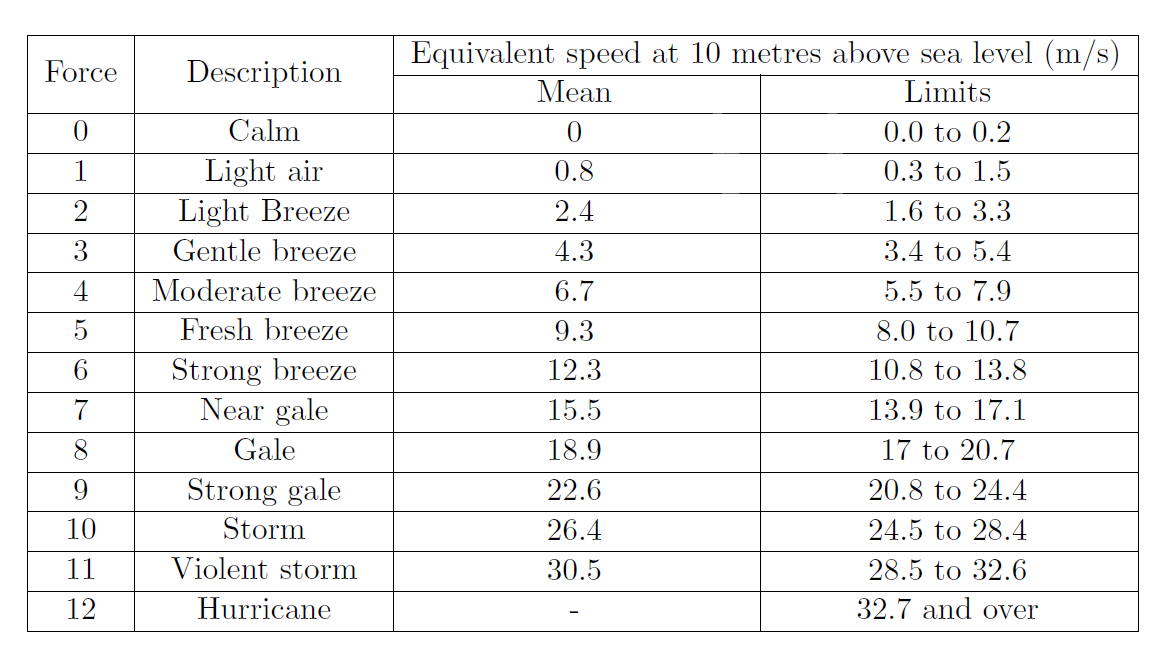
\includegraphics[width=1\textwidth]{images/Tabla Beaufort Efect.png}
    \caption{Escala Beaufort}
     Fuente: \cite{BeaufortScale2012}
     \label{tabla:escala_beaufort}
\end{figure}


\newpage


\subsection{Búsqueda del valor óptimo de la torsión}

Se procede a probar un caso estándar en el que se presentan las siguientes variables globales y algunos aspectos que se comentados a lo largo de la Sección \ref{section:2_desarollo_cálculo}: 

\begin{itemize}
  \item Número de palas = 1
  \item Número de segmentos = 5
  \item Longitud de la pala $L$ = 75 (m)
  \item Densidad de la pala = 1176 $(Kg/m^3)$
  \item Grosor de la pala = 20\%
  \item Diámetro de la góndola = 4 (m)
  \item CP, obtenido mediante la Figura \ref{fig:coef_potencias_6MW}
  \item Ángulo de cabeceo $\theta_1$ = 2 ($^{\circ}$)
  \item $J_{left}$ = 3 (m)
  \item $J_{right}$ = 0.6 (m)
  \item Ancho Buje = 2 (m)
  \item Ancho Buje = 0.25 (m)


\end{itemize}


En un primer momento se pensó hacer un ejemplo en el que sin ángulo de cabeceo se demostrase la importancia de la torsión con respecto a la obtención de energía. Pero como se comentó en el Desarrollo teórico, es necesario contar con una pala realista para que se genere una fuerza de sustentación y así generar energía. \\

Además, estableciendo un ángulo de cabeceo estático también es posible demostrar la importancia de la torsión como efecto y cuantitativamente.\\

Se procede a estudiar un primer ejemplo, este está generado para velocidades de viento en la escala de Beaufort de entre 0 y 10 de fuerza, aunque el tramo más importante de obtención de energía se encuentra entre los niveles 5 y 6. Además añadir, que para vientos de fuerza 0-2 la generación de potencia es nula debida al peso de las palas y la fuerza que se debe generar para producir fuerzas de giro en la pala.

\begin{figure}[H]
    \centering
    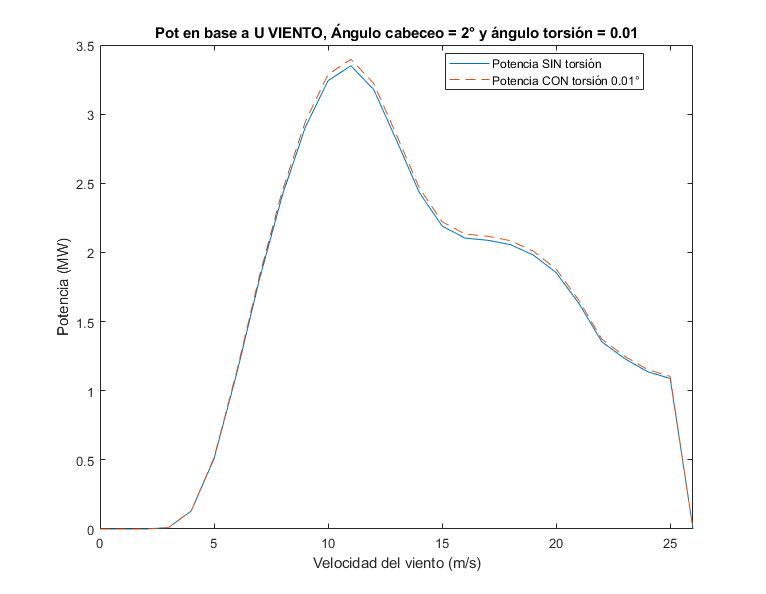
\includegraphics[width=1\textwidth]{images/0-10beau CP bueno.png}
    \caption{Potencia obtenida con viento de entre 0 y 1 de fuerza según la escala Beaufort}
     \label{fig:0-10beaufort_primertest}
\end{figure}

Observando la Figura \ref{fig:0-10beaufort_primertest} se puede vislumbrar la pequeña diferencia que supone haber torsionado las palas únicamente 0.1$^{\circ}$ por segmento. Además, parece que en el caso de hacer ampliar la representación la diferencia entre las potencias cada vez es menor.\\

Se realiza el análisis de la eficiencia basándonos en la anterior figura para comprobar si la hipótesis planteada resulta ser correcta. Se procede a obtener el valor de la eficiencia para algunos valores de velocidad del viento (4-25 $\dfrac{m}{s}$) lo suficientemente espaciados para observar el espectro completo:

\begin{table}[H]
\centering
\begin{tabular}{c|cccccccc|}
\cline{2-9}
\multicolumn{1}{l|}{} &
  \multicolumn{8}{c|}{Ángulo de cabeceo $\theta_1$ = 2$^{\circ}$ y Ángulo de torsión $\Delta_\theta$ = 0.1$^{\circ}$} \\ \hline
\multicolumn{1}{|c|}{Velocidad viento (m/s)} &
  \multicolumn{1}{c|}{4} &
  \multicolumn{1}{c|}{7} &
  \multicolumn{1}{c|}{10} &
  \multicolumn{1}{c|}{13} &
  \multicolumn{1}{c|}{16} &
  \multicolumn{1}{c|}{19} &
  \multicolumn{1}{c|}{22} &
  25 \\ \hline
\multicolumn{1}{|c|}{Eficiencia, $\eta$} &
  \multicolumn{1}{c|}{1.0139} &
  \multicolumn{1}{c|}{1.0139} &
  \multicolumn{1}{c|}{1.0139} &
  \multicolumn{1}{c|}{1.0139} &
  \multicolumn{1}{c|}{1.0139} &
  \multicolumn{1}{c|}{1.0139} &
  \multicolumn{1}{c|}{1.0139} &
  1.0139 \\ \hline
\end{tabular}
    \caption{Eficiencia del rotor en función de la velocidad del viento}
     \label{tabla:eficiencia_primer_intento}
\end{table}

La suposición era correcta, la relación entre las potencias es constante. Esto puede llegar descolocar de cierta manera uno de los pensamientos iniciales cuando se comenzó este trabajo, ya que se pensaba o se podía imaginar que a mayor cantidad de viento la torsión tendría mas efecto sobre el rotor y las palas. Pero en base a una sola prueba no se puede pensar que se está en lo cierto. \\


A continuación se probarán ángulos de torsión $\Delta_\theta$ entre 0.01 y 0.04$^{\circ}$ crecientes hacia el final de la pala, manteniendo el ángulo de cabeceo $\theta_1$.

\begin{figure}[H]
    \centering
    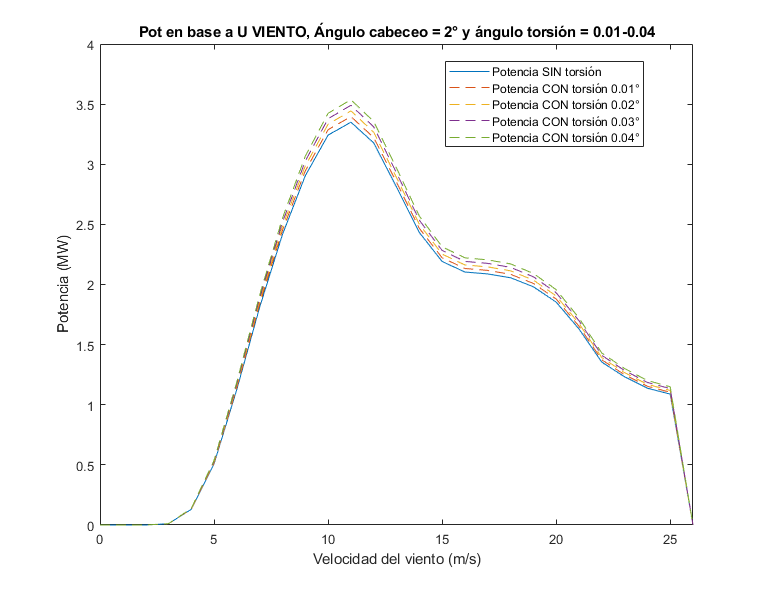
\includegraphics[width=1\textwidth]{images/0-10beau CP bueno 001-004.png}
    \caption{Potencia obtenida para $\Delta_\theta$ entre 0.01 y 0.04$^{\circ}$ }
     \label{fig:beau_torsion_001-004}
\end{figure}

A simple vista parece que los resultados que se han obtenido ahora que se ha torsionado son mejores. Se pasa a comprobar si la eficiencia obtenida para el caso en el cual cada segmento torsiona 0.04 ($^{\circ}$).

En este caso la eficiencia obtenida es 1.0559, se trata de una mejora del 5\% en la obtención de energía, lo cual puede llegar a suponer un alto beneficio a lo largo del tiempo.\\

El sistema generado para esta sección podría seguir mejorando la obtención de energía mediante mas torsión ya que no se han generado impedimentos para ello. Diversos trabajos estudian los efectos de la torsión, como el realizado por José-Félix en 2009 \cite{funes2009analisis} , este se trata de un amplio estudio relacionado con el estudio simplificado de palas. En él se estudia el efecto de la torsión y como afecta a las palas y a su deformación, puesto que cuanto más se torsione una pala antes se deteriorará, esto también ocurre cuando a las palas se les aplica el efecto conocido como \textit{bending}.\\

En el trabajo anteriormente mencionado se explica que la torsión debe decrecer a lo largo que incrementa la longitud de la pala para maximizar la obtención de energía, debido a que la velocidad de arrastre ( $v_{arrastre} = \Omega \cdot brazo_i$ ) provoca el incremento de la torsión de la pala según aumenta el radio.


\begin{figure}[H]
    \centering
    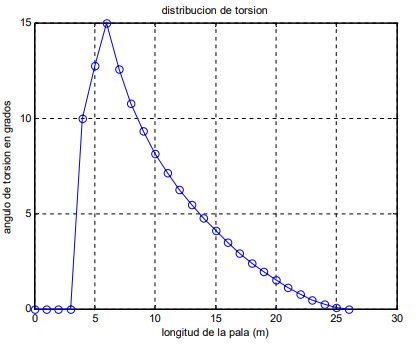
\includegraphics[width=0.8\textwidth]{images/distribución torsión.PNG}
    \caption{ Ángulos de torsión a lo largo de la longitud de la pala }
    Fuente: PFC \cite{funes2009analisis}, Figura 3.5
     \label{fig:torsion_decrece_radio}
\end{figure}

En la Figura se muestra que los 3 primeros metros no se presenta torsión y esto es debido a que la pala presenta una zona de unión del buje con el rotor, en nuestro caso la obviamos.\\

Se prueba un sistema de torsión parecido y posteriormente uno invertido a este como el que se explicó en la Ecuación \ref{def:theta_cte}. Respetando las porciones del apartado, para alcanzar una torsión de 15$^{\circ}$ se deberá torsionar cada segmento 3$^{\circ}$.


\begin{figure}[H]
    \centering
    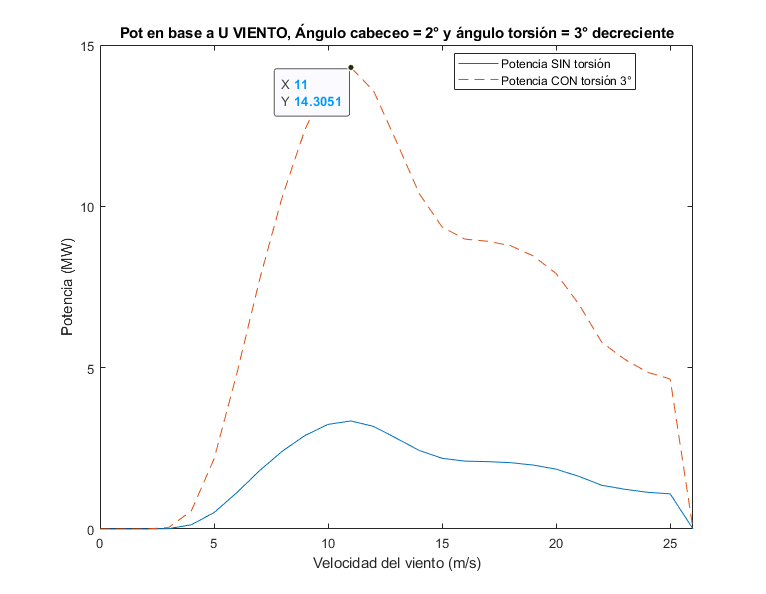
\includegraphics[width=1\textwidth]{images/torsion 3 decreciente.png}
    \caption{Potencia generada por un ángulo de torsión = 15$^{\circ}$ que decrece 3$^{\circ}$ por segmento}
     \label{fig:torsion_decrece3}
\end{figure}

Se deja como referencia la potencia en caso de no torsionar la pala para comprender la capacidad de mejora que tiene la torsión con respecto a no tenerla. Destacar que la potencia obtenida en estos casos se aleja considerablemente de la realidad debido a la suposición de un ángulo de ataque de 2$^{\circ}$ constante para con la pala. El ángulo de ataque cambia continuamente a causa de los giros que realiza el rotor.




Ahora se obtiene la potencia para el caso en el que el ángulo de torsión crece:
\begin{figure}[H]
    \centering
    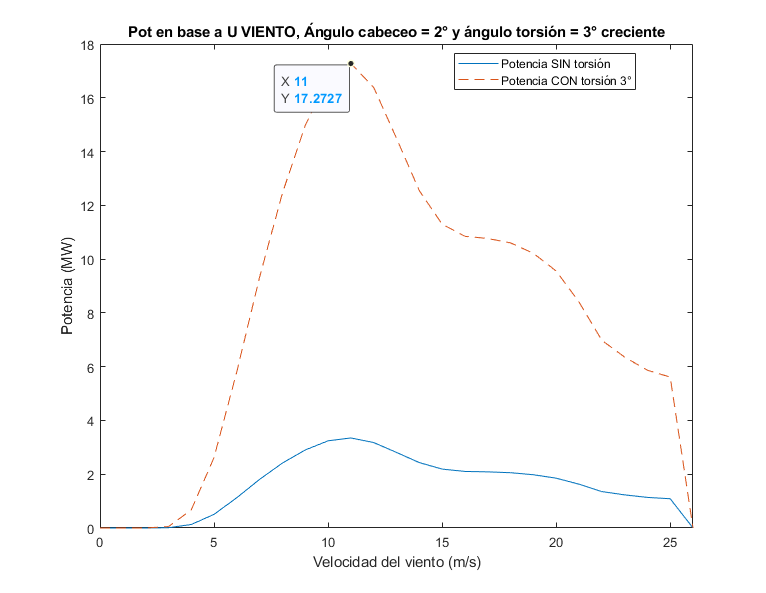
\includegraphics[width=1\textwidth]{images/torsion 3 creciente.png}
    \caption{Potencia generada por un ángulo de torsión = 15$^{\circ}$ que crece 3$^{\circ}$ por segmento}
     \label{fig:torsion_crece3}
\end{figure}

Se ha obtenido una mayor cantidad de potencia usando el método que se expuso a lo largo de este trabajo. En cuanto a la eficiencia se obtiene 5.1565, un factor de mejora desorbitado. Obteniendo más de 5 veces la potencia inicial en caso de que no existiera torsión.\\

\subsection{La torsión como efecto perjudicial}

Esta sección trabajará con el mismo conjunto de variables globales que se usaron en la anterior.\\

Con pequeños o medianos valores de torsión únicamente se ha obtenido mejora de los valores de potencia, pero también es posible que esta se convierta en un problema.\\

Además, en este trabajo dividimos la pala en cinco segmentos, lo que supone un problema de torsión mayor que si la hubiéramos dividido por un número de segmentos más alto. Eso se debe a que los segmentos tienen un gran tamaño y si se giran grandes ángulos pueden llegar a suponer un bloqueo del viento que está entrando al sistema.\\

\begin{figure}[H]
    \centering
    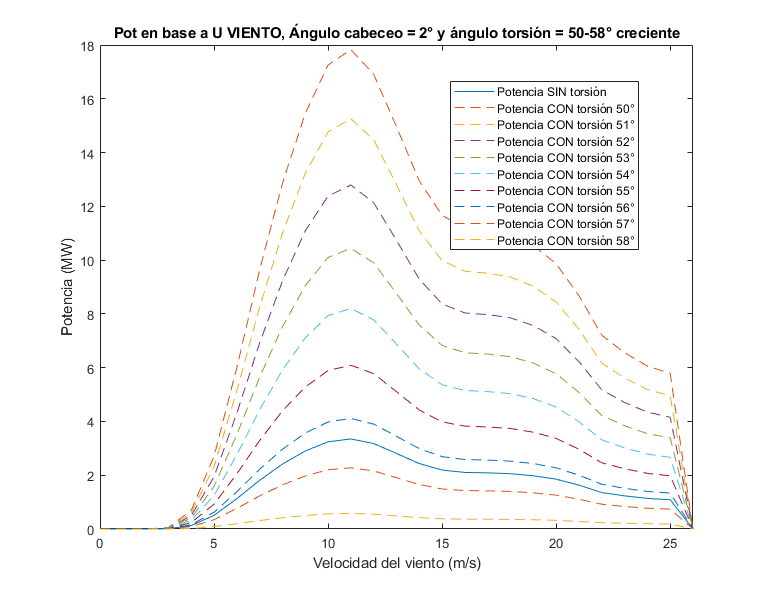
\includegraphics[width=1\textwidth]{images/torsion 50-58 creciente.png}
    \caption{Potencia generada por un ángulo de torsión = 50-58$^{\circ}$ aplicado a cada segmento}
     \label{fig:torsion_crece50-58}
\end{figure}

Observando la Figura \ref{fig:torsion_crece50-58} se puede observar que entre los valores 56-58$^{\circ}$ de torsión por segmento se comienza a descompensar la influencia positiva de la torsión para pasar a obtener valores de potencia menores que los obtenidos en el caso de que la pala fuera completamente plana con tan solo 0.17 de eficiencia.\\


Las palas imaginadas para este ejemplo son irreales e irrealizables en la vida real y probablemente acabasen partiéndose o partiendo la torre del aerogenerador debido a la tensión que podrían llegar a generar sobre el rotor.